\chapter{Existence and Absence of Hopf Bifurcation in Phosphorylation-Dephosphorylation CRN}

\section{What even \textbf{is} a bifurcation?}
To better generalize them, it'd be best to also define the notion of:
\begin{definition}	
	\textbf{Invariant sets}. \footcite{faye2011Bifurcation} \footcite{afrajmovich1999Bifurcation}

	Taking the Auton. sys.
	\begin{equation}\label{invar_set_auton_sys}
		\dot{y} = f(y) , y(0) = y_0, y \in \mathbb{R}^n
	\end{equation}

	A state-set $S \subseteq \mathbb{R}^n$ of \ref{invar_set_auton_sys} is \textbf{invariant} if $\forall y_0 \in S, \forall t \geq 0: y(t) \in S$
\end{definition}

As you can see by this above definition, equilibria are also particular cases of invariant sets, themselves.

They also fall into stability classes that can be defined as in Def. \ref{equilibrium_stability}, but replacing
\[
	"y_0" \text{ with } "S \subseteq \mathbb{R}^n \text{ }"
\]
and
\[
	" \dotso \norm{y(t) - y_0} \dotso" \text{ with } "\dotso \text{ inf}\{ \norm{y(t) - s} : s \in S  \} \dotso \text{ }"
\]
The Jacobian (linearization), generally, would also not be as useful in this context anymore.
\newpage
Now consider we have a system as above, except it now depends on an extra parameter $\mu$, which remains constant \textbf{during} our "experiment".
\begin{equation}\label{auton_parameter_sys_compact}
	\dot{y} = f_\mu(y).
\end{equation}

This could be, for example, the length of the pendulum $L$, in \ref{damped_pendulum}, or its damping coefficient $c$. Honestly generalizing it even more, it could even be the gravitational constant $g$. Hence, this parameter can, of course be a \textbf{vector} of such parameters.

The way the parameter $\mu$ varies also induces variations in the topology and dynamics of the system. That's obvious since this is kind of the point of parameters in systems.

What can vary though can be trivial or more interesting.

The positions of invariant sets, for example can vary continuously

during changes in $\mu$; that's usually normal.

But what's more interesting is when these change their \textbf{stability} altogether, equilibria disappear completely / appear out of thin-air - or, even - collide with other invariant sets.

This odd behavior is called a \textbf{bifurcation}, and $\mu$, in this case is a \textbf{bifurcation parameter}.

The former types of bifurcations I talked about previously are called \textbf{local}, those in which changes in stability can only be considered mostly for \textbf{isolated equilibria}, individually, or other invariant sets whose stability can be analyzed \textbf{locally}, via the system's linearization at a point.

The latter are \textbf{global}, which are more complex and require greater understanding of the system beyond a local linearization, but that falls into the special-case category described in the last paragraphs of the previous chapter, and so far all I know about Mr. Prof. Lyapunov as of now is that his brother was a pianist. But thankfully our interest for this work lies with local bifurcations, so we'll be ignoring this for now, maybe I'll come back to it during my Master's (not).

To better define and illustrate them for the 1-D case and give example of bifurcations for such dimension, we could instead write our vector field $f$ as depending on $\mu$ in addition to the unknown function $y$.
\begin{equation}\label{eq:1-d_bif_sys}
	\dot{y} = f(y, \mu).
\end{equation}
And assume $f \in C^k(\mathbb{R} \bigtimes \mathbb{R}), k \geq 2 $ around $(0,0)$, and
\begin{equation}\label{bifurcation_priming}
	f(0,0) = 0, \quad \frac{\partial f}{\partial y}(0,0) = 0.
\end{equation}
By these conditions we are basically "priming" the system for bifurcations, but none are enough for them to actually occur. Here come the specific definitions for each particular type of bifurcation in 1-D.

\begin{definition}
	A \textbf{Saddle-node bifurcation}:
	for $f$ in \ref{bifurcation_priming}, add as well:
	\begin{equation*}
		\frac{\partial f}{\partial \mu}(0,0) =: a \neq 0, \quad \frac{\partial^2 f}{\partial y^2}(0,0) =:b \neq 0.
	\end{equation*}
\end{definition}
Then, for \ref{eq:1-d_bif_sys}, a saddle-node bifurcation occurs at $\mu = 0$, if the following equivalences are true:

\rom{1}. For $ab < 0$ (resp. $ab> 0$), $\nexists y : f(y,\mu) = 0$ for $\mu < 0$ (resp. $\mu > 0$)

\rom{2}. For $ab < 0$ (resp. $ab > 0$), $\exists y_+(\epsilon) \neq y_-(\epsilon) \implies y_\pm(\epsilon) : f(y_\pm(\epsilon), \mu) = 0, \epsilon = \sqrt{\abs{\mu}}$, for $ \mu > 0 $ (resp. $\mu < 0$), having opposing stabilities.

\begin{definition} \label{pitchfork_bif}
	\textbf{Pitchfork bifurcation}.

	For $f$ from \ref{bifurcation_priming}, assume as well that:
	$f \in C^k, k \geq 3$,
	\[
		f(-y, \mu) = -f(y,\mu)
	\]
	and,
	\[
		\frac{\partial^2 f}{\partial \mu \partial y}(0,0) =: a \neq 0, \quad \frac{\partial^3 f }{\partial y^3}(0,0)=: b \neq 0
	\]

	Now, a \textbf{pitchfork bifurcation} occurs for \ref{eq:1-d_bif_sys} at $\mu  =0$ if:

	\rom{1}. for $ab < 0$ (resp. $ab > 0$) $\exists! y = 0 :f(y,\mu) = 0 $ for $\mu < 0$ (resp. $\mu > 0$). $b < 0 \implies$ stable, $b > 0 \implies$ unstable.

	\rom{2}. for $ab < 0$ (resp. $ab > 0$) $\exists y = 0 : f(y , \mu) = 0$, as well as: $y_+(\epsilon) \neq y_-(\epsilon) \implies y_\pm(\epsilon) : f(y_\pm(\epsilon), \mu) = 0, \epsilon = \sqrt{\abs{\mu}}$  for $\mu > 0$ (resp. $\mu < 0$), for which $y_+(\epsilon) = -y_-(\epsilon)$, Both $y_-(\epsilon)$ and $y_+(\epsilon)$ have matching stabilities, whereas $y = 0$ has the opposite stability of them, given by $b < 0 \implies$ stable, $b > 0 \implies$ unstable.
\end{definition}

\begin{definition}
	\textbf{Transcritical bifurcation}.

	For $f$ in \ref{bifurcation_priming}:
	\[
		\frac{\partial^2 f}{\partial \mu \partial y}(0, 0) =:a \neq 0, \quad \frac{\partial^2 f}{\partial y^2}(0,0) =: b \neq 0
	\]
	Then a \textbf{transcritical bifurcation} occurs for \ref{eq:1-d_bif_sys} at $\mu = 0$, char. by (if they hold):

	\rom{1}.  $\exists y = 0 : f(y, \mu) = 0$  and  $ \exists y_0(\mu) : f(y_0(\mu), \mu) = 0 $ where $\mu \rightarrow u_0(\mu) \in C^m, m = k - 2$

	\rom{2}.  for $a\mu  < 0$ (resp. $a\mu > 0$) the trivial fixed point $y = 0 \implies$ stable (resp. unstable)
	and $u_0(\mu)$ has opposing stability.
\end{definition}

Finding local bifurcations can be done by looking at eigenvalues.
\newpage
{\large The local bifurcation condition

}For system:
\begin{equation}
	\dot{y} = f(y, \mu) \quad f : \mathbb{R}^n \times \mathbb{R} \rightarrow \mathbb{R}^n
\end{equation}

\begin{definition}\label{local_bif_def}
	$(y_0,\mu_0)$ admits a \textbf{local bifurcation} if:
\end{definition}

If $\forall \lambda \in Eig(J_{f}(y_0,\mu_0)) : Re(\lambda) \leq 0$, while $\exists \lambda_0 : Re(\lambda_0) = 0$

\begin{equation}\label{stable_state_bif}
	\text{If } \lambda_0 = 0 \text{ the bifurcation is stable-state defined. }
\end{equation}

We also have a second kind of local bifurcation and this is where we begin the crux of the thesis, and answer the first question I had getting into this:

\section{What is a simple Hopf Bifurcation?}

A \textit{simple Hopf bifurcation} is a bifurcation in which a single complex-conjugate pair of eigenvalues of the Jacobian matrix crosses the imaginary axis, while all other eigenvalues remain with negative real parts. Such a bifurcation generates nearby oscillations or periodic orbits.

Or, more formally, defined similarly to Def. \ref{local_bif_def}:
\begin{definition}
	$(y_0, \mu_0)$ admits a \textbf{Hopf bifurcation} if we have Def. \ref{local_bif_def}, and additionally:
	\begin{equation}\label{hopf_bif_def}
		\exists! \lambda_0 : Re(\lambda_0) = 0, \quad
		Im(\lambda_0) \neq 0.
	\end{equation}
\end{definition}
Visually, just to hammer it in:

\begin{figure}[H]
	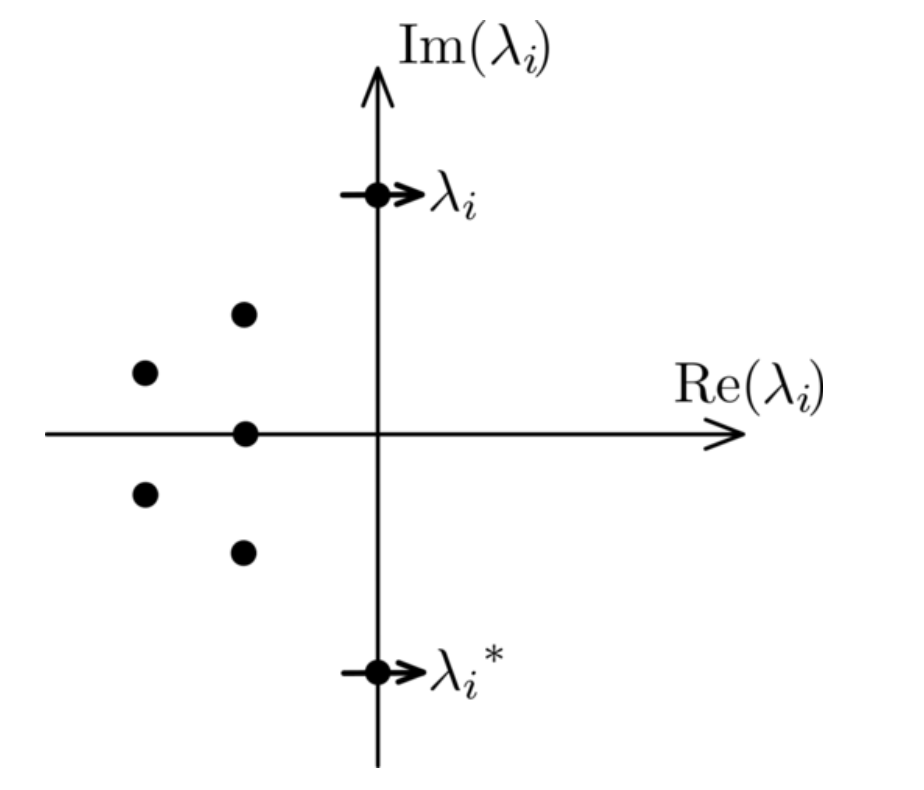
\includegraphics[width=13cm]{math_pics/hopf-bif-eigenvalue-graph.png}
	\centering
	\caption{Visualizing the zeroes \footcite{vogel2020HopfEigenvalues}}
\end{figure}

In $\mathbb{R}^2$, such Bifurcations cause special kinds of invariant sets, namely \textbf{limit cycles} to appear. These are periodic solutions, for which we'll need a few more concepts in order to be able to define them:
\begin{definition} \textbf{Closed trajectory and Closed orbit (cycle)}

	A trajectory (or flow): $y(t) \in \mathbb{R}^2$ as in Def. \ref{dyn_sys_orbit_flow_etc_def} is a solution for \ref{eq:1-d_bif_sys}

	A closed trajectory is one which returns to its starting point $\forall s_0 := \Phi(0,s) $ it has, namely:
	\begin{gather*}
		\exists t_0 \in T : \Phi(t,s) = \Phi(t+t_0,s), \forall s \in \Phi_{s_0}     \\
		\Updownarrow \\
		\exists t_0 \in T : y(t) = y(t+t_0), \forall t \in T
	\end{gather*}
	A \textbf{closed orbit} or \textbf{cycle} is just the image of such a closed trajectory.
\end{definition}

\begin{definition}\textbf{Limit point}
	These can be grouped into $\omega$ (attracting) and $\alpha$ (repelling) limit points:

	$y_\omega$ is an $\omega$-limit point  for $y$ if:

	$\exists (t_n)_{n \in \mathbb{N}} \subseteq I(y) : $
	\begin{gather*}
		\lim_{n \rightarrow \infty} t_n = \infty  \\
		\lim_{n \rightarrow \infty} \Phi(t_n,y) = y_\omega
	\end{gather*}
	And similarly, but in reverse:

	$y_\alpha$ is an $\alpha$-limit point  for $y$ if:

	$\exists (t_n)_{n \in \mathbb{N}} \subseteq I(y) : $
	\begin{gather*}
		\lim_{n \rightarrow \infty} t_n = \textbf{--} \infty  \\
		\lim_{n \rightarrow \infty} \Phi(t_n,y) = y_\alpha
	\end{gather*}
\end{definition}

\begin{definition}\textbf{Limit set}
	The set of all $\omega$ (or $\alpha$)-limit points for a particular orbit $\gamma$ is called the \textbf{limit set} of $\gamma$, denoted and defined as:
	\[
		\lim_{\omega}\gamma_s := \bigcap_{t \in T} \overline{ \{ \Phi(t', s) : t' > t \} }
	\]
	\[
		\lim_{\alpha}\gamma_s := \bigcap_{t \in T} \overline{ \{ \Phi(t', s) : t' < t \} }
	\]
\end{definition}

\begin{definition} \textbf{Limit cycle}(finally)

	A Limit Cycle is a cycle which is the limit set of at least another trajectory.
	Also, interestingly:
	\[
		\lim_{\omega}\gamma \bigcap \gamma  = \emptyset \implies \text{ it's an } \omega \text{-limit cycle}.
	\]
	\[
		\lim_{\alpha}\gamma \bigcap \gamma  = \emptyset \implies \text{ it's an } \alpha \text{-limit cycle}.
	\]
\end{definition}

What's interesting though, and makes calculations easier for the 2-D case is:
\begin{theorem}  \textbf{Poincaré-Bendixson}

	For a dynamical system $(T,X,\Phi)$ with $X \subseteq \mathbb{R}^2$, $\forall$ compact invariant set $S$:
	\begin{gather*}
		\text{if } \nexists x_0 \in S : \Phi(t_1, x_0) = \Phi(t_2,x_0), \forall t_1,t_2 \in T \\
		\Downarrow \\
		\forall s \in S: \gamma_s \text{ are either limit cycles, or } \lim_{\omega / \alpha}\gamma_s \text{ is an $\omega$ (or $\alpha$)-limit cycle }.
	\end{gather*}
\end{theorem}

But the problem is this theorem only holds for $\mathbb{R}^2$. For higher dimensions we don't have this property necessarily, instead we have to look for periodic solutions (limit cycles) ourselves - which, as stated previously - occur naturally during a Hopf bifurcation.

So having these in mind, Hopf is kind of like an $\mathbb{R}^n$ version of Pitchfork bif.: \ref{pitchfork_bif} when you think about it.

You can even see the resemblance in the way they look \footcite{brainsci10080536}

\begin{figure}[H]
	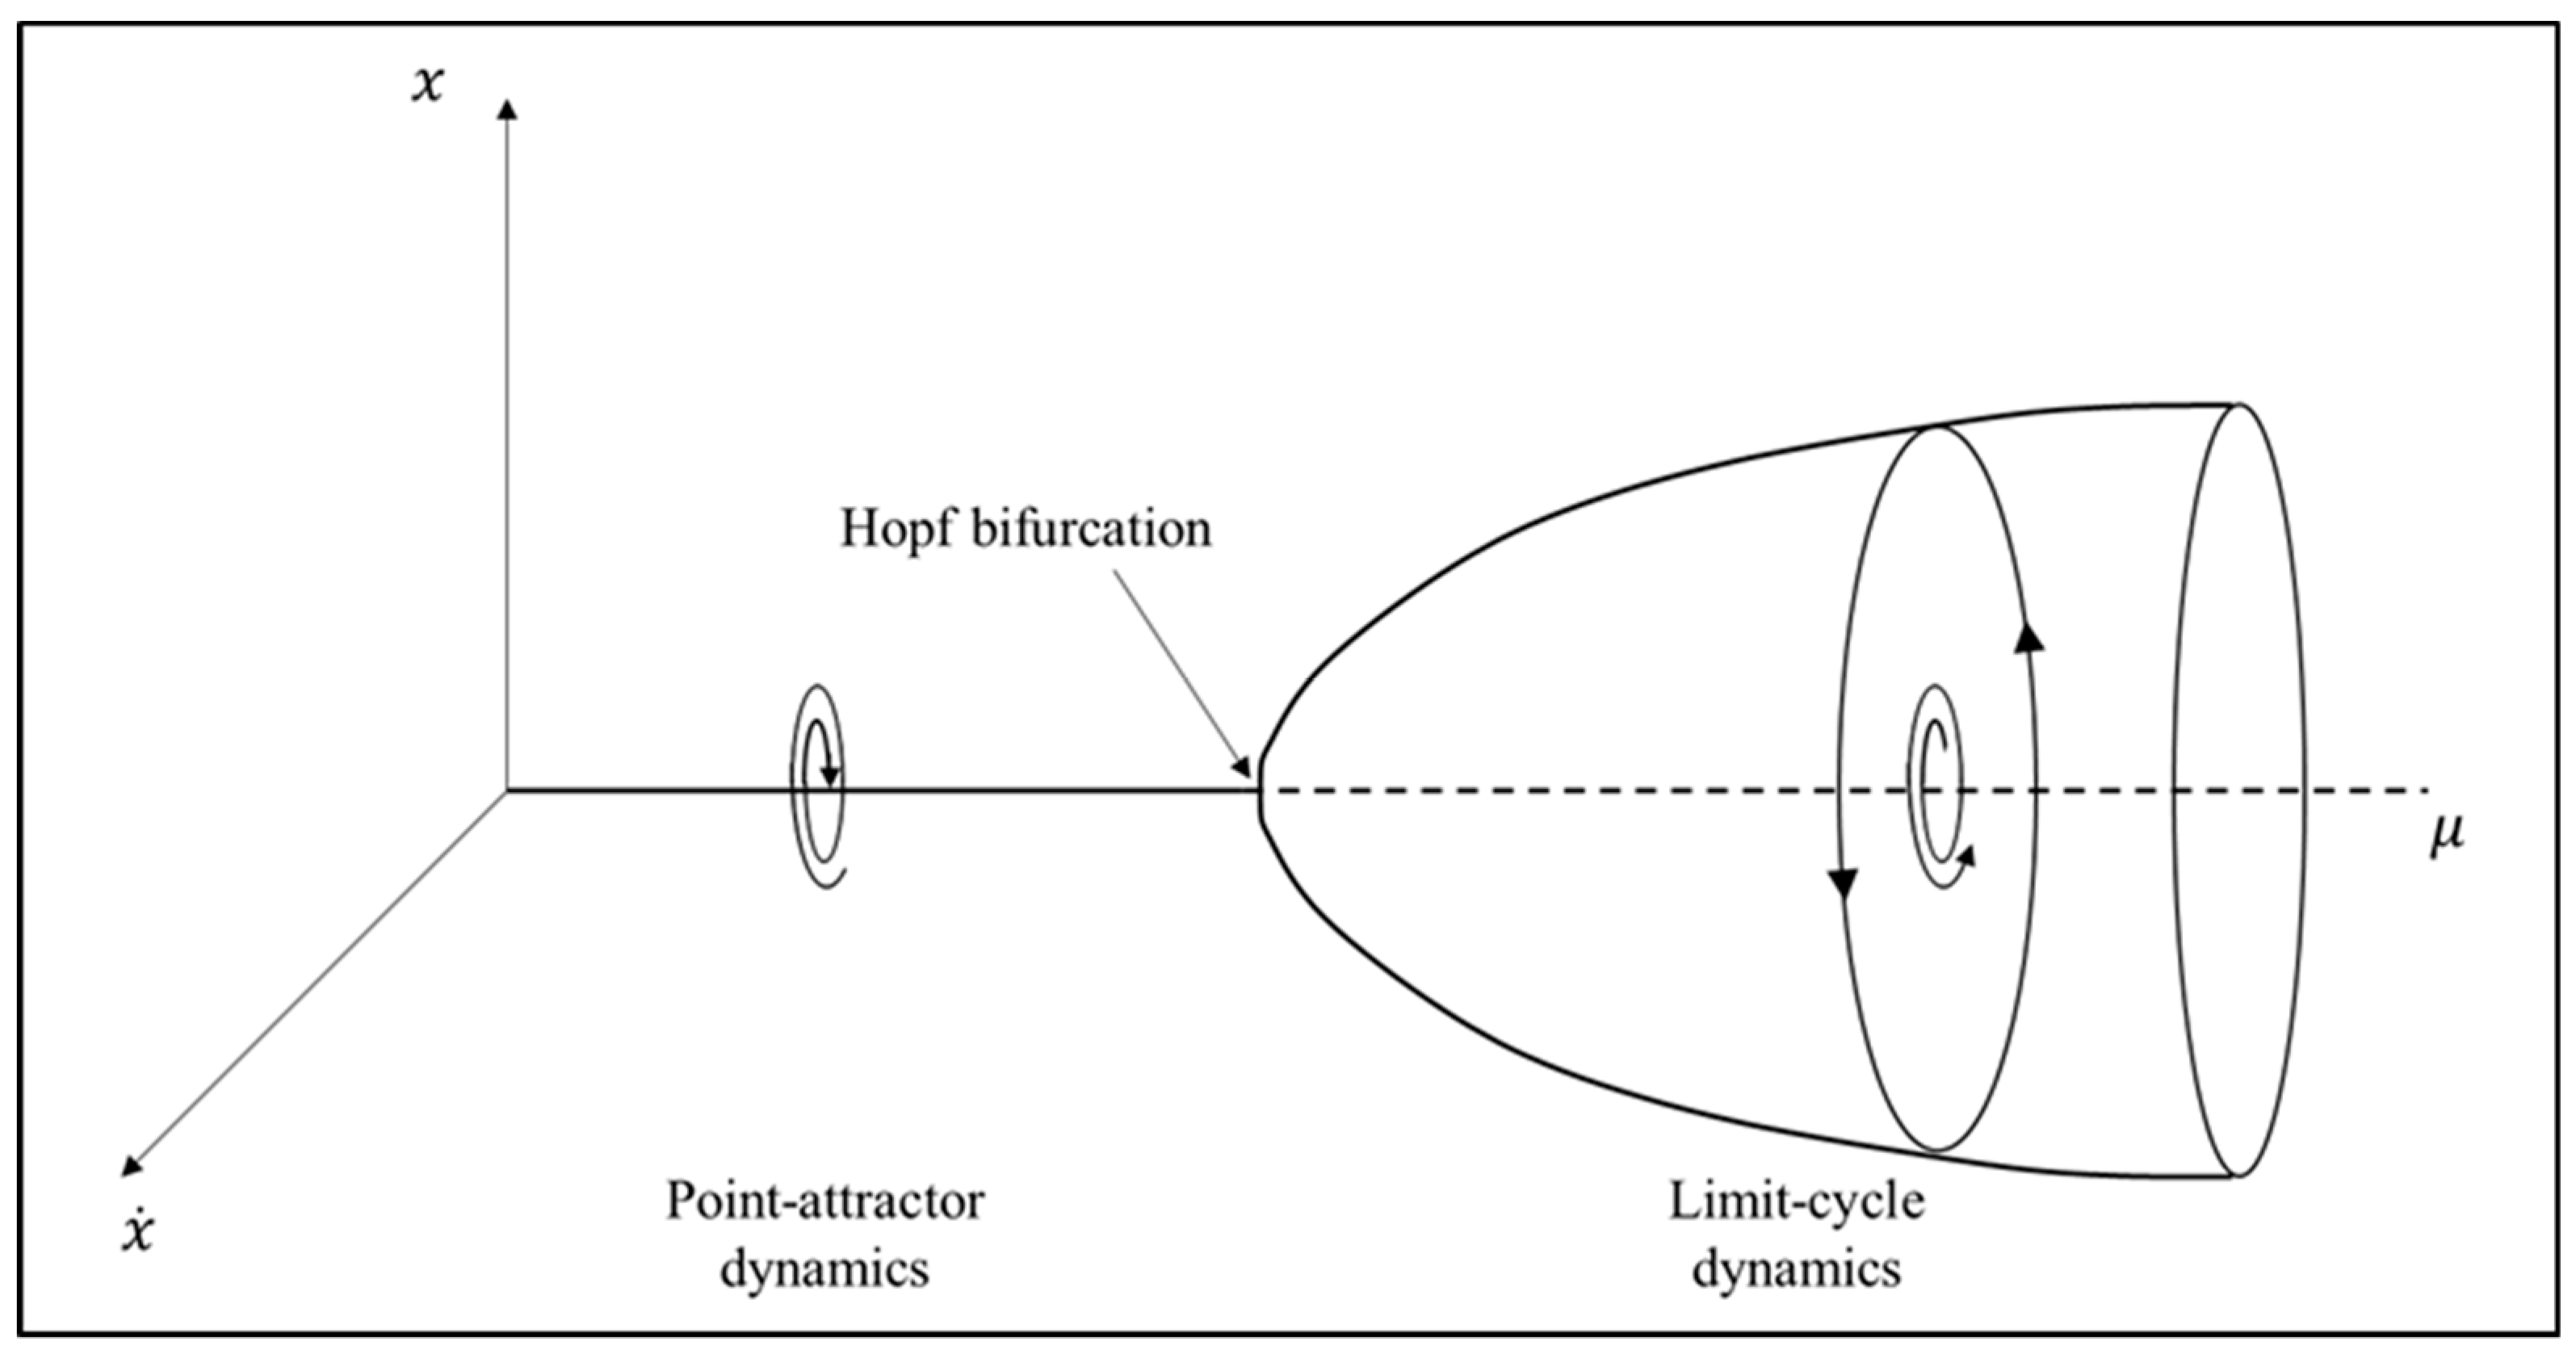
\includegraphics[width=13cm]{math_pics/hopf-bif-pic.png}
	\centering
\end{figure}

\begin{figure}[H]
	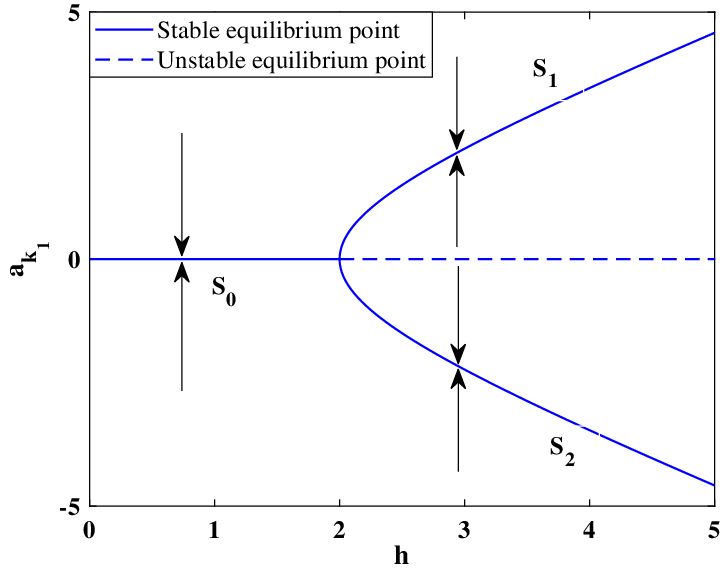
\includegraphics[width=13cm]{math_pics/pitchfork-photo.png}
	\centering
	\caption{Pitchfork bifurcation \cite{Yang2020}}
\end{figure}

\subsection{Proving the existence of simple Hopf bifurcations}

Finding necessary conditions for their existence makes use of a tool defined in the previous chapter (\ref{hurwitz_theorem}) the \textbf{Hurwitz matrix}. \footcite{LIU1994250}

Instead, now the characteristic polynomial depends on this new bifurcation parameter $\mu$.

\begin{proposition}\label{symmetric_roots_pair_criterion}
	Take $p_{\mu_0} \in \mathbb{C}^n[Z]$ with $n \geq 2$ and consider $\mu_0$ fixed:
	\[
		p_{\mu_0}(z) = a_0(\mu_0)z^n + a_1(\mu_0)z^{ n-1 } + \dots + a_n (\mu_0)
	\]

	Take $H_i(\mu_0)$ to be $p$'s $i$-th Hurwitz Matrix (\ref{hurwitz_theorem})

	If we have:
	\begin{gather*}
		\det H_1(\mu_0) > 0 , \dots, \det H_{n-2} (\mu_0) > 0. \\
		\Downarrow \\
		\text{ pair of symmetric roots of   } p_{\mu_0}(z) \leq 1
	\end{gather*}

	And $\exists!$ pair of symmetric roots $\iff \det H_{n-1}(\mu_0) = 0$.

	If $a_n(\mu_0) > 0 \implies$ for the pair $\lambda_i, \overline{\lambda_i}$  : Re$(\lambda_i) =$ Re$(\overline{\lambda_i}) = 0$.
\end{proposition}

Now, more specifically, the necessary conditions for a simple Hopf bifurcation are:

\begin{proposition}\label{yangs_criterion}
	\cite{Yang2002}
	A simple Hopf bifurcation occurs at fixed point $x^*$ and at the parameter threshold $\mu_0$ $\iff$
	\begin{gather*}
		\rom{1} \quad \det  H_{ n-1 }(\mu_0) = 0 \text{  and  } a_s(\mu_0) > 0, \\
		\rom{2} \quad 		\det H_1(\mu_0) > 0 , \dots, \det H_{n-2} (\mu_0) > 0 \text{  and  } \\
		\rom{3} \quad \left. \frac{d(\det H_{n-1}(\mu))}{d\mu} \right|_{\mu = \mu_0} \neq 0.
	\end{gather*}
\end{proposition}

\subsection{Ruling out simple Hopf bifurcations}

Directly from criterion \ref{symmetric_roots_pair_criterion} we have a criterion for showing $\nexists \mu$ for which $x(\mu)$ undergoes simple Hopf bifurcations.
\begin{theorem}\label{ruling_out_simple_hopf_bif}

	For the dynamical system $\dot{x} = f_\mu(x)$ assume $\exists$ a curve of steady states $x(\mu)$.
	$p_\mu(z)$ is the characteristic polynomial of degree $s \geq 2$ of the linearization $J(x(\mu), \mu)$, and $H_i(\mu)$ its $i$-th Hurwitz matrix. Given:
	\[
		\det H_1(\mu_0) > 0 , \dots, \det H_{n-2} (\mu_0) > 0. \forall \mu
	\]
	And either:
	\begin{gather*}
		a_s(\mu) \leq 0 \text{ whenever  } \det H_{s-1} = 0  \\
		\text{or} \\
		\det   H_{s-1}(\mu) \neq 0, \forall \mu    \\
		\Downarrow
	\end{gather*}
	$\nexists$ simple Hopf bifurcation $\forall \mu$ at the steady states $x(\mu)$.
\end{theorem}

\subsection{Convex parameters}\label{convex_paramteres}
\footcite{ErramiEtAl2015a} \footcite{Rockafellar1973}
With most dynamical systems, if we want to analyze their behavior we have to find, through all possible values if $\exists x^*(\mu)$ fixed points for which bifurcation occur, and hence we need to find any value $\exists \mu$ of the bifurcation parameter for which said bifurcation occurs, throughout our entire domain.

But luck would have it, though that the kind of systems we care about in this thesis, namely chemical reaction systems, defined in more detail in \ref{mass-action_network}, are not like "most" dynamical systems.

They all have a certain structure and their corresponding differential equations look in a way that can be represented more manageably.

Take now a system for a CRN, written as well in its matrix form, as in \ref{crn_system_matrix_form}
\[
	\dot{x} = f(k,x) :=\Gamma v(k,x)
\]
Where $v$, the flux vector, as in \ref{flux_vector} can be written as:
\[
	v(k, x) = \text{diag}(k)\Psi(x).
\]
as well.
Where diag $: \mathbb{C}^n \rightarrow \mathcal{M}_n(\mathbb{C})$,
\begin{align*}
	(\text{diag}(x))_{i,i} = x_i, \quad \forall i = \overline{1,n} \\
	(\text{diag}(x))_{i,j} = 0, \quad \forall i,j = \overline{1,n} , i \neq j.
\end{align*}
And $\Psi(x)$ is the flux vector, where the reaction rates \ref{reaction_rate} are written without the leading $k_i$'s, only depending on $x$.

If we want to look into how the system behaves near equilibrium points $x^*$ we have to, just like other systems, study their Jacobian matrix, which, because the flux vector is made of polynomials can be written using this little trick:
\[
	J(k, x)_{\mid x=x^*}=\Gamma \operatorname{diag}\left(v\left(k, x^*\right)\right) \Gamma_L^T \operatorname{diag}\left(\frac{1}{x^*}\right)
\]

Now since $x^*$ is a fixed point, the flux vector satisfies:
\begin{equation}\label{flux_vector_linear_problem}
	\Gamma v(k,x^*) = 0, \quad v \geq 0.
\end{equation}
And so the solutions of (\ref{flux_vector_linear_problem}) (ker$\Gamma$) are vectors (rays) which describe a \textbf{convex polyhedral cone} \footcite{dattorro2018Convex} called the \textbf{flux cone}.

It's been shown in (\cite{clarke1980stability}) that:

$(k,x^*)$ satisfies \ref{flux_vector_linear_problem} $\iff  v(k,x^*)\in \text{ker}(\Gamma) \bigcap \mathbb{R}^r_{\geq 0}$

Where $r:$ no. of reactions.

A flux cone is expressed as an $\mathbb{R}_{\geq 0}$ linear combination (positive hull) of its extreme vectors $\left\{ E_1 , \ldots , E_l \right\}$. Also, we need $E_i \neq 0_r, \forall i = \overline{1,l}$

\begin{definition}\label{convex_params_definition}
	\textbf{Convex parameters.}
	\begin{equation}\label{flux_cone}
		\boxed{		v=\sum_{i=1}^l \lambda_i E_i=E \lambda, \quad \lambda_i \geq 0, \forall i = \overline{1,l} }
	\end{equation}
	Where $\lambda_i$ are called \textbf{convex parameters}.
\end{definition}
But we also need something to parametrize the $x$'s, so:
\begin{equation}\label{other_convex_parameters}
	\boxed{	h_i=\frac{1}{x_i^*}, \quad i = \overline{1,n} }
\end{equation}
So having this in mind:
\begin{definition}
	A convex parameter vector:
	\[
		(h, \lambda) = (h_1, \ldots, h_n , \lambda_1, \ldots , \lambda_l) \in \mathbb{R}_{>0}^n \times \mathbb{R}_{\geq 0}^{l} : E \lambda \in \mathbb{R}^r_{> 0}.
	\]
	With $E$ the matrix whose columns are the convex polyhedral cone's extreme vectors.
\end{definition}
So we may write the Jacobian using this new coordinate system, which in turn makes its coefficients monomials, instead of the usual polynomial and multiple-term expressions you usually get with these systems, like in Ex. (\ref{bigger_network_example1}).
\newcommand\eqCuzConvex{\stackrel{\mathclap{\normalfont\mbox{\ref{flux_vector_linear_problem}, \ref{convex_params_definition}}}}{=\joinrel=\joinrel=\joinrel=\joinrel=}}

\begin{gather}\label{jacobian_convex_params}
	v(k, x^*) \eqCuzConvex E \lambda  \notag \\
	\Downarrow \text{ \ref{other_convex_parameters} } \notag \\
	\boxed{J(k,x)_{|x=x^{*}}=J(h,\lambda)=\Gamma \text{diag}(E\lambda)\Gamma_{L}^{T}\text{diag}(h)}
\end{gather}

We could, of course turn this convex vector back into the regular coordinate system:

Given:
\begin{gather}\label{k_convert_back_from_convex}
	(h,\lambda) \Downarrow \notag \\
	\text{Let  } x^* \in \mathbb{R}^n , \boxed{
		x^*_i = \frac{1}{h_i} , i = \overline{1,n}
	} \notag \\
	\boxed{
		k = \text{diag}(\Psi(h)) E \lambda \in \mathbb{R}^r_{> 0}
 }
\end{gather}

There is one particular case that is of interest to us, though.

\section{What is a Phosphorylation-Dephosphorylation CRN?}

Phosphorylation of proteins occurs in cycles, which are fueled by $3$ proteins which are the ingredients: a substrate $S$ and $2$ enzymes: kinase ($K$) and phosphatase ($F$).

The one that starts this chain is the kinase ($K$), attaching phosphate groups onto the substrate, phosphorylating it.

Then, phosphatase ($F$) comes in and undoes all the hard work kinase ($K$) put in and removes the phosphate groups, now dephosphorylating the substrate.

\hfill\break
These cycles are a particular case of a broader type of what are called \textbf{posttranslational modification (PTM) systems.} \footcite{conradi2024} Another example would be, for instance \textbf{methylation}, where in this case methyl groups are the ones attaching to specific sites. \footcite{ramazi2021Ptms, SCHOENHEIMER1939333}

The reason we care about them is their key implication in \textbf{ signal transduction}, which is the process our cells use to communicate with one-another. Any disturbance in this system is linked to its own class of health complications in our body. \footcite{CONRADI2018507, 10.1093/hmg/ddp186, cohen2001Phosphorylation}

Basically, do these biochemical systems induce periodic solutions as in (\ref{hopf_bif_def}), likening clocks, or do they have multiple steady-states (\textbf{capacity for bistability}), likening switches?

What these all have in common, though are the \textbf{building blocks} used to create them:
\begin{equation}\label{ptm_building_blocks}
	S+M \xrightleftharpoons[k_2]{k_1} SM \xrightarrow{k_3} S^* + M \quad \mathrm{~and~} \quad S^* + U \xrightleftharpoons[k_5]{k_4} S^* U \xrightarrow{k_6} S + U
\end{equation}

What's familiar to the previous example is the presence of a substrate ($S$), which forms the \textbf{complex} ($SM$) with the \textbf{modifier} ($M$), which - as the name implies - modifies ($S$) to become ($S^*$), which then dissociates with ($M$);

And just like in dephosphorylation, another modifier ($U$) can come in and undo the entire hustle ($M$) did.

So the \textbf{phosphorylation version of this would be}:
\begin{gather*}\label{phosphorylation_reaction_basis}
	S_0 + K \xrightleftharpoons[k_2]{k_1} K S_0 \xrightarrow{k_3} S_1 + K  \xrightleftharpoons[k_5]{k_4} \ldots K S_{n-1} \xrightarrow{k_{ 3n}} S_n + K  \\
	\text{ for the phosphorylation side, and} \\
	S_n + F \xrightleftharpoons[k_{2(n+1)}]{k_{2n+1}} F S_n \xrightarrow{k_{2n + 3}} S_{n-1} + F  \xrightleftharpoons[k_{2n + 5}]{k_{2n + 4}} \ldots F S_{1} \xrightarrow{k_{6n}} S_0 + F  \\
	\text{ for the dephosphorylation side, and}
\end{gather*}
Which phosphorylates the substrate ($S$) up to a certain number of phosphate groups $n$, and then \textbf{de}phosphorylates it back to 0, where the subscript notation $S_i ;  i = \overline{1,n}$ represents the substrate ($S$) with its $i$ phosphate groups.

\subsection{Cyclic and mixed distributive and processive Phosphorylation-Dephosphorylation CRN}
The system above represents a \textbf{distributive} cycle, meaning each bounding site of ($K$) and ($F$) (de)phosphorylate only one single phosphate group.

As opposed to a \textbf{processive} one, which would look something like:
\begin{equation*}
	S_0 + K \xrightleftharpoons[k_2]{k_1} S_0 K \xrightarrow{k_3} S_1 K \xrightarrow{k_4} S_2 + K
\end{equation*}
For a binding one, and
\begin{equation*}
	S_2 + F \xrightleftharpoons[k_2]{k_1} S_2 F \xrightarrow{k_3} S_1 F \xrightarrow{k_4} S_0 + F
\end{equation*}
For the unbinding operation.

Notice these extra reactions where the enzymes don't dissociate.
\begin{gather*}
	\ldots S_0 K \xrightarrow{k_3} S_1 K \xrightarrow{k_4} \ldots \\
	\ldots S_2 F \xrightarrow{k_3} S_1 F \xrightarrow{k_4} \ldots	
\end{gather*}

It was shown that processive systems are globally stable and distributive ones may be bistable (having multiple steady states).

There are also extra classifications in double phosphorylation systems:

The order phosphorylation occurs matters too, so if:
\rom{1}: the \text{last} phosphorylated site is being dephosphorylated in the first dephosphorylation binding, then the mechanism is said to be \textbf{sequential}.

\rom{2} Whereas, if the \text{first} phosphorylated site is being \textbf{de}phosphorylated first then the system is \textbf{cyclic}.

You can see here an example of this classification in two mechanisms that, while they differ in this category, they are still both distributive.\footcite{conradi2024}
\begin{figure}[H]	
	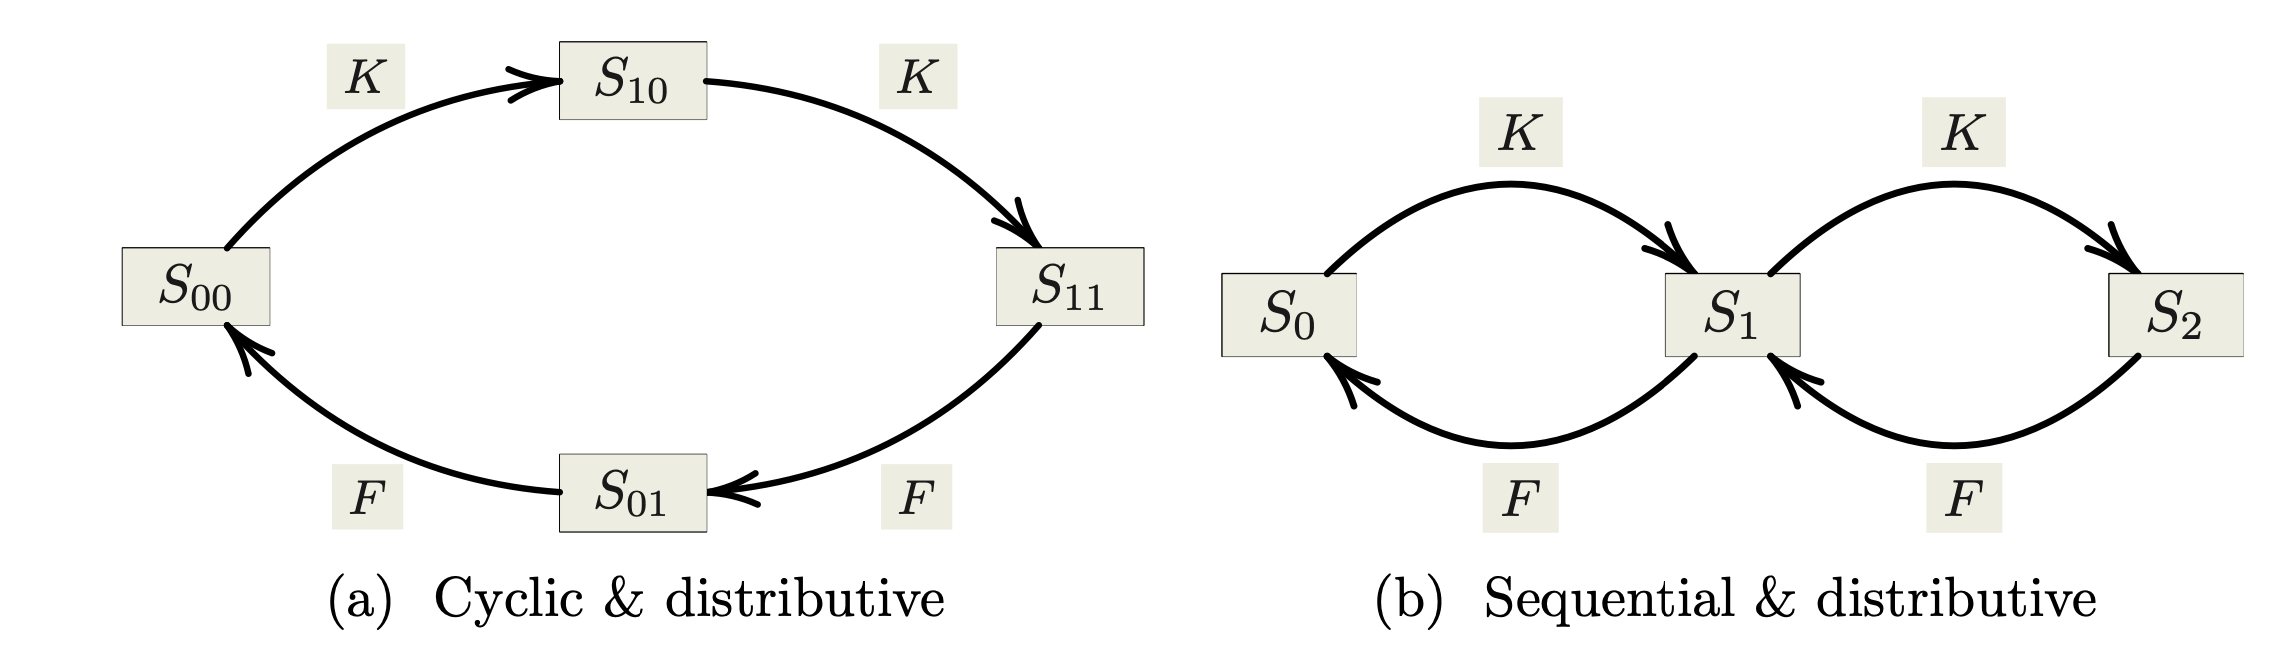
\includegraphics[width=13cm]{math_pics/cyclic-vs-sequential.png}\label{cyclic_vs_sequential_figure}
	\centering
\end{figure}
In the left one here, $S_{ij}$ shows which one of the $2$ binding sites gets phosphate groups attached to it, (Ex, $S_{10}$: first one is phosphorylated, second not).

We'll now try to solve the problem whether a particular system undergoes simple Hopf bifurcations.

Take, for example, the following basic cycle:

\textbf{Example 1} $(\mathcal{N}_1)$:
\begin{figure}[H]
	\centering
	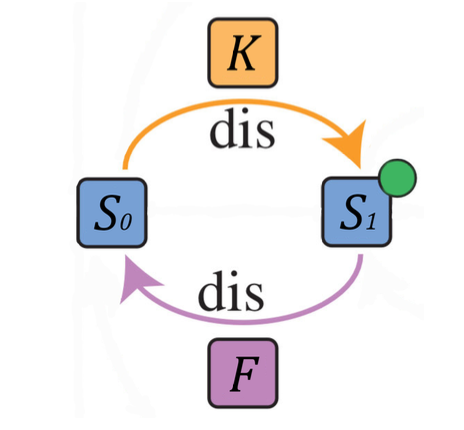
\includegraphics[width=38mm]{math_pics/ex1-no-bifurcations.png}	
	\caption{Network $( \mathcal{N}_1 )$ \footcite{doi:10.1098/rsif.2014.1405}}
\end{figure}

Whose chemical reaction notation looks like:
\begin{gather}\label{network1}
	K + S_0 \xrightleftharpoons[k_2]{k_1} K S_0 \xrightarrow{k_3} K + S_1 \tag{$\mathcal{N}_1$} \\
	F + S_1 \xrightleftharpoons[k_4]{k_5} F S_1 \xrightarrow{k_6} F + S_0 \notag
\end{gather}

\textbf{Remark 1:} $(a)$ As you can see, the network (\ref{network1}) consists of $6$ species ($2$ substrates $S_0$, $S_1$; $2$ enzymes $K$, $F$; which together form $2$ complexes: $K S_0$, $F S_1$) and $6$ reactions ($2$ reversible and $2$ irreversible) with matrix subspace $=$ rank $\Gamma = 3$.

Using \href{https://github.com/viktorashi/Open-CoNtRol}{the app}, talked more about in Chap.\ref{ch:web-app}, I've generated the following stoichiometric matrices, its rank and its corresponding dynamical system:

\begin{align*}
	\Gamma &=
	\begin{pmatrix}
		K & -1 &  1 &  1 &  0 &  0 &  0 \\
		S0& -1 &  1 &  0 &  0 &  0 &  1 \\
		KS0 &  1& -1& -1 &  0 &  0 &  0 \\
		S1 &  0 &  0 &  1& -1 &  1 &  0 \\
		F &  0 &  0 &  0& -1 &  1 &  1 \\
		FS1 &  0 &  0 &  0 &  1& -1& -1  \\		
	\end{pmatrix}, \quad \text{rank}(\Gamma) = 3 \\[3ex]
	\Gamma_L &=
	\begin{bmatrix}
		1&0&0&0&0&0\\
		1&0&0&0&0&0\\
		0&1&1&0&0&0\\
		0&0&0&1&0&0\\
		0&0&0&1&0&0\\
		0&0&0&0&1&1
	\end{bmatrix} \\[3ex]
	&
	\begin{cases*}
		\begin{array}{ll}
			\dot{x}_1(t) = -k_4 x_1(t) *x_6(t)+k_5 x_2(t)+k_6 x_2(t) \\
			\dot{x}_2(t) = k_4 x_1(t) *x_6(t)-k_5 x_2(t)-k_6 x_2(t) \\
			\dot{x}_3(t) = -k_1 x_3(t) *x_5(t)+k_2 x_4(t)+k_3 x_4(t) \\
			\dot{x}_4(t) = k_1 x_3(t) *x_5(t)-k_2 x_4(t)-k_3 x_4(t) \\
			\dot{x}_5(t) = -k_1 x_3(t) *x_5(t)+k_2 x_4(t)+k_6 x_2(t) \\
			\dot{x}_6(t) = k_3 x_4(t)-k_4 x_1(t) *x_6(t)+k_5 x_2(t) \\
		\end{array}	
	\end{cases*}
\end{align*}
Where the "species to index mapping" is:
\[
	F:  x_1
 | FS1: x_2
 | K: x_3
 | KS0: x_4
 | S0: x_5
 | S1: x_6
\]
\textbf{Remark 1:} $(b)$ For the network (\ref{network1}), the cone (defined as in \ref{flux_cone}) $\Gamma v(k,x) = 0, \forall v \geqq 0$ is spanned by the vectors $w_0, w_1, w_2 \geqq 0 : \lambda_0 w_0 + \lambda_1 w_1 + \lambda_2 w_2 \geqq 0 \iff \lambda_1, \lambda_2, \lambda_3 \geq 0$.

Now we may consider the Jacobian written in convex parameters for network (\ref{network1}), $J_1(h,\lambda)$ as defined in \ref{jacobian_convex_params}, which is parametrized by $9$ parameters: $\lambda_0, \lambda_1, \lambda_2$ and $h_1, \ldots, h_6$.

So, from \textbf{Remark 1} $(a)$ and $(b)$, it follows that the characteristic polynomial of $J_1(h, \lambda)$ is
\[
	p_{h,\lambda}(z) = z^3 (a_0(h,\lambda) z^3 + a_1(h, \lambda)z^2 + a_2 (h,\lambda)z + a_3(h,\lambda) )
\]
Where each coefficient $a_i, i = \overline{0,3}$ depends on these $9$ parameters.

Now, with the motivation of (\ref{ruling_out_simple_hopf_bif}) in mind, we compute the values of $a_i(h,\lambda), i = \overline{0,3}$ and $\det H_i(h,\lambda), i = \overline{1,2}$ according to (\ref{hurwitz_theorem}), obtaining the following proposition:
\begin{proposition}
	Based on the notation above, for the network (\ref{network1}):

	$\det H_1(h,\lambda)$, $\det H_2(h,\lambda)$ and $a_3(h,\lambda)$ contain only positive monomials. Thus, $\det H_1(h,\lambda)$, $\det H_2(h,\lambda) \geq 0, \forall h, \lambda \geqq 0$, specifically $\det H_2(h,\lambda) \neq 0$, $\lightning$ (\ref{ruling_out_simple_hopf_bif}).
\end{proposition}
\begin{proof}
	Now to solve these we're going to use some Maple scripts that rely on the \cite{franz2016ConvexMaple} package (too large to include inside this document).

	Given the network structure defined above, as well as the $E\lambda$ matrix made of the extreme cone vectors (\textbf{ray}):
	\[
		E\lambda =
		\begin{bmatrix}
			\lambda_2 + \lambda_3 \\
			\lambda_1 \\
			\lambda_3 \\
			\lambda_2 + \lambda_3 \\
			\lambda_2 \\
			\lambda_3
		\end{bmatrix}
	\]
	The Jacobian in convex parameters, as given in (\ref{jacobian_convex_params}), using that script is:
	\[
		\left. J_1(h,\lambda)=
		\left[
			\begin{array}{ccccccc}-\lambda_1hl&-\lambda_1h2&0&0&0&0&\lambda_1h7\\-\lambda_1hl&-\lambda_1h2&\lambda_1h3&0&0&0&0\\\lambda_1hl&\lambda_1h2&-\lambda_1h3&0&0&0&0\\0&-\lambda_2h2&\lambda_1h3&(-\lambda_2-\lambda_1)h4&0&\lambda_2h6&0\\0&\lambda_2h2&0&\lambda_2h4&-\lambda_2h5&0&0\\0&0&0&0&\lambda_2h5&-\lambda_2h6&0\\0&0&0&\lambda_1h4&0&0&-\lambda_1h7
		\end{array}\right.\right]
	\]
	Then by means of another Maple script, we can write the Hurwitz matrices of its corresponding characteristic polynomial. (They are pretty huge and will always overflow \LaTeX, you can find more about them in \ref{appendix})

	\hfill\break
	//TODO : pune appendixu cu coadele de maple sau macar mentionandu-le
	\hfill\break

	But just by looking at $H_2(h,\lambda)$, we can deduce that $a_{ij}$ is a positive monomial, for all  its entries $\forall h , \lambda > 0$, in particular $\det H_2(h, \lambda) \neq 0$.

	So, $\det H_1(k,x^*) > 0, \forall k, x^* > 0$, moreover the coefficient of the largest degree term in the characteristic polynomial $a_3(k, x^*) > 0$, so according to \ref{ruling_out_simple_hopf_bif} : For network (\ref{network1}), $\nexists k, x^* \geqq 0$ for which $J_1(k,x^*)$ has a pair of purely imaginary eigenvalues $\implies \nexists$ a simple Hopf bifurcation in our system for any rate constants or positive steady states
\end{proof}

\textbf{Example 2}:
Here we'll show how to prove the \textbf{existence} of a Hopf bifurcation in a network, which requires quite a bit of a lot of work.\footcite{conradi2024, Suwanmajo2020, Conradi2020} Let us take the cyclic example, Network $(a)$ from \ref{cyclic_vs_sequential_figure}, from which we can actually infer a particular case of networks with some nice properties.

We'll first need to define some continuations of convex parameters \ref{convex_params_definition}, aided by \ref{hurwitz_theorem} in regard to this particular case.

\hfill\break
\subsection{The Jacobian of networks with a single extreme vector}\label{jacobian_single_extreme_vector}

If (\text{no. of extreme rays}) $l = 1 \implies$ the cone ker$(\Gamma) \bigcap \mathbb{R}^r_{\geq 0}$ is spanned by a single extreme vector, so the Jacobian can be written more simply in terms of just it, and its corresponding scalar $\lambda$, in convex coordinates.
\begin{equation}\label{jacobian_convex_single_extreme_ray}
	J_\lambda(h)=\lambda \Gamma \operatorname{diag}(E)\Gamma_L^T\operatorname{diag}(h).
\end{equation}
Where its char. poly. is:
\begin{equation}\label{char_poly_j_lambda}
	\det(\mu I-J_\lambda(h))=\mu^{n-s}(\mu^s+a_1(\lambda,h)\mu^{s-1}+\ldots+a_s(\lambda,h))
\end{equation}
With $s := \text{rank}(J_\lambda) \leq n$.
But for the particular case $\lambda = 1$:
\begin{equation}\label{char_poly_j_1}
	\det(\mu I-J_1(h))=\mu^{n-s}(\mu^s+b_1(h)\mu^{s-1}+\ldots+b_s(h))
\end{equation}
Now we'll use a Corollary (the consequence of a Lemma discussed in another more in-depth section) to relate the general $\lambda > 0$ case with the $\lambda = 1$ case.
\begin{corollary}
	Let's say $E \in \mathbb{R}^r_{\geq 0}$. Let $J_\lambda(h)$ as in \ref{jacobian_convex_single_extreme_ray} with

	rank$(J_{\lambda}(h))=\mathrm{rank}(J_{1}(h))=s<n$ and $a_i(\lambda,h), b_i(h)$ coeff. of \ref{char_poly_j_lambda} and \ref{char_poly_j_1}. $\implies$
	\begin{equation}\label{colorally_jacobians_1st_satisfaction}
		a_i(\lambda,h)=\lambda^ib_i(h),i=1,\ldots,s.
	\end{equation}
	aaand
	\begin{equation}\label{colorally_jacobians_2nd_satisfaction}
		\begin{aligned}\det(\mu I_n-J_\lambda(h))&=\det(\mu I_n-\lambda J_1(h))\\&=\mu^{n-s}\lambda^s\left(\left(\frac{\mu}{\lambda}\right)^s+\sum_{i=1}^sb_i(h)\left(\frac{\mu}{\lambda}\right)^{s-i}\right)
		\end{aligned}
	\end{equation}
\end{corollary}
Sooo: \textbf{Remark: }

\rom{1} From \ref{colorally_jacobians_2nd_satisfaction} $\implies$ for $\omega(h) \in \text{Eig}(J_1(h)) \implies \mu(\lambda, \omega) = \lambda \omega(h) \in \text{Eig}(J_\lambda)(h)$.

\rom{2} $\mathrm{sign}(Re(\mu(\lambda,h)))=\mathrm{sign}(Re(\omega(h)))$

\rom{3} $J_\lambda(h)$ has an $\mu \in$Eig with Re$(\mu) = 0$ of the form $\pm i \lambda w(h) \iff J_1$ has one of the form $\pm i \omega (h)$.

Now, utilizing this result, along with \ref{yangs_criterion}, we may find sufficient conditions for bifurcations in single ray-defined networks

Constructing Hurwitz determinants:
\begin{gather*}
	H_l(\lambda, h) \text{of \ref{colorally_jacobians_1st_satisfaction}} \\
	\text{and} \\
	G_l(h) \text{of \ref{colorally_jacobians_2nd_satisfaction}}
\end{gather*}

\begin{proposition}
	We get the following relationship:
	\[
		\det\left(H_l(\lambda,h)\right)=\lambda^{l(l+1)/2}\det\left(G_l(h)\right),l=\overline{1,s}
	\]
	So we basically only need \ref{colorally_jacobians_2nd_satisfaction} and to study the $G_i(h), i = \overline{1,s}$ Hurwitz matrices if the system's convex polyhedral cone ker$\Gamma \bigcap \mathbb{R}^r_{\geq 0}$.
\end{proposition}
\begin{proposition}
	For $\dot{x} = \Gamma v(k,x)$, ODE system for CRN with mass-action kinetics, rank$(\Gamma) = s$. Suppose the Matrix E from \ref{convex_params_definition} is a single extreme ray, and the Jacobian $J_\lambda(h)$ is as in \ref{jacobian_convex_single_extreme_ray}.
	Also, let the char. polynomials of $J_\lambda(h)$ and $J_1(h)$ be as in \ref{char_poly_j_lambda} and \ref{char_poly_j_1}, respectively.

	If $\exists h = h^* :$
	\[
		\begin{aligned}
			b_s(h^*)&\mathrm{>0~and}\\\det(G_1(h^*))&>0,...,\det(G_{s-2}(h^*))>0\mathrm{and}\\\det(G_{s-1}(h^*))&=0,
		\end{aligned}
	\]
	then:

	\rom{1} $J_1(h^*)$ has a single pair of purely imaginary eigenvalues $\mu = \pm i \omega(h^*)$.

	\rom{2} $J_\lambda(h^*)$ has a single pair of purely imaginary eigenvalues $\mu = \pm i \lambda \omega(h^*), \forall \lambda > 0$.

	\rom{3} for $\dot{x} = \Gamma v(k,x), \exists$ simple Hopf	 bifurcation at $h = h^*$, $\forall \lambda > 0$ if $\exists i \in \left\{ 1 , \ldots , n \right\}:$
	\[
		\frac{\partial\det(G_{n-1})}{\partial h_i}|_{h_i=h_i^*}\neq0.
	\]
	Meaning, it crosses the axis at that point.
\end{proposition}
Hence, because $\det(H_{s-1}(h,\lambda))=\lambda^{\frac{s(s-1)}{2}}\det(G_{s-1}(h))$, $\lambda$ is not a well-suited bifurcation parameter, since $\frac{\partial\det(H_{s-1}(h,\lambda))}{\partial\lambda}|_{h=h^{*}}=0$ when $\det(G_{s-1}(h^{*}))=0$. It all basically comes down to $h$, not $\lambda$.
\hfill\break

Now, let's get into the bread of it. We may re-define the cyclic and distributive system we're going to discuss again.
\begin{figure}[H]
	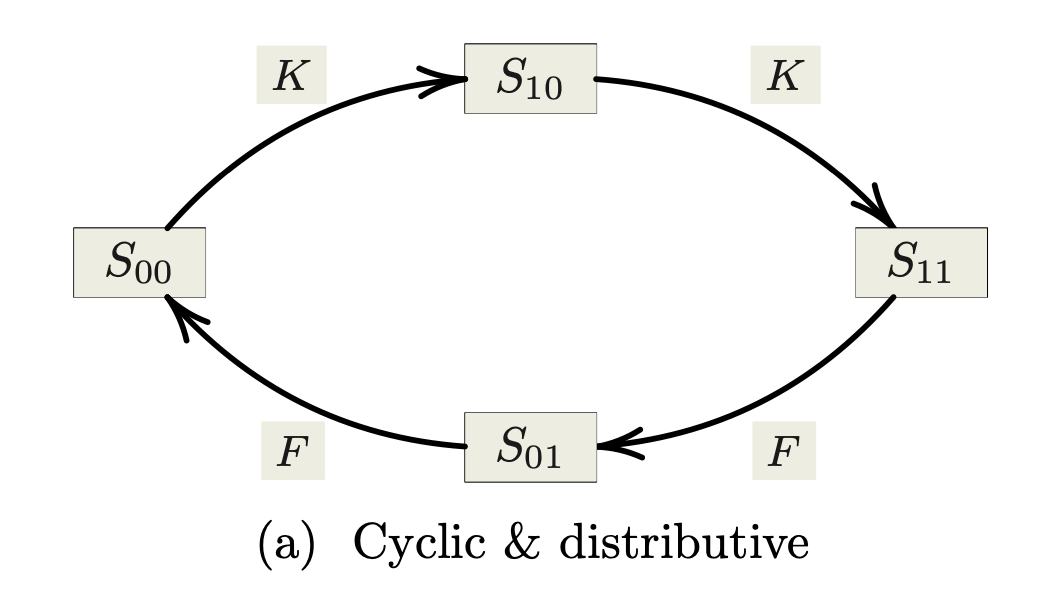
\includegraphics[width=13cm]{math_pics/cyclic-distributive-n1.png}	
	\centering
	\caption{$\mathcal{N}_2$ \footcite{conradi2024}}
\end{figure}
Defined by these reactions:
\begin{align}\label{network2}
	S_{00} + K \xrightleftharpoons[ k_2 ]{k_1} KS_{00} \xrightarrow{k_3} S_{10} + K \xrightleftharpoons[ k_5 ]{k_4} KS_{10} \xrightarrow{k_6} S_{11} + K \tag{$\mathcal{N}_2$}
	\\
	S_{11} + F \xrightleftharpoons[ k_8 ]{k_7} FS_{11} \xrightarrow{k_9} S_{01} + F \xrightleftharpoons[ k_{11} ]{k_{10}} FS_{01} \xrightarrow{k_{12}} S_{00} + F \ \notag
\end{align}
We'll look into just the irreversible sub-network, though.
\begin{align}\label{network2_irr}
	S_{00} + K \xrightarrow{k_1} KS_{00} \xrightarrow{k_3} S_{10} + K \xrightarrow{k_4} KS_{10} \xrightarrow{k_6} S_{11} + K \tag{$\mathcal{N}_2 / IR$}
	\\
	S_{11} + F \xrightarrow{k_7} FS_{11} \xrightarrow{k_9} S_{01} + F \xrightarrow{k_{10}} FS_{01} \xrightarrow{k_{12}} S_{00} + F \ \notag
\end{align}
And using the following index-to-species mapping:
\[
	\begin{array}{ccccccccccc}x_{1}&x_{2}&x_{3}&x_{4}&x_{5}&x_{6}&x_{7}&x_{8}&x_{9}&x_{10}\\K&F&S_{00}&S_{10}&S_{01}&S_{11}&KS_{00}&KS_{10}&FS_{01}&FS_{11}
	\end{array}
\]
We may obtain their system of ODEs:

$\mathcal{N}_2$:
\[
	\begin{aligned}
		\dot{x}_1&=-k_{1}x_{1}x_{3}-k_{4}x_{1}x_{4}+(k_{2}+k_{3})x_{7}+(k_{5}+k_{6})x_{8}\\\dot{x}_2&=-k_{10}x_{2}x_{5}-k_{7}x_{2}x_{6}+(k_{8}+k_{9})x_{10}+(k_{11}+k_{12})x_{9}\\\dot{x}_3&=-k_1x_1x_3+k_2x_7+k_{12}x_9\\\dot{x}_4&=-k_4x_1x_4+k_3x_7+k_5x_8\\\dot{x}_5&=-k_{10}x_2x_5+k_9x_{10}+k_{11}x_9\\\dot{x}_6&=-k_7x_2x_6+k_8x_{10}+k_6x_8\\\dot{x}_7&=-(k_2+k_3)x_7+k_1x_1x_3\\\dot{x}_8&=-(k_5+k_6)x_8+k_4x_1x_4\\\dot{x}_9&=-(k_{11}+k_{12})x_9+k_{10}x_2x_5\\\dot{x}_{10}&=-(k_8+k_9)x_{10}+k_7x_2x_6
	\end{aligned}
\]
$\mathcal{N}_2 / IR$:
\[
	\begin{aligned}
		\dot{x}_{1} &= -k_{1} x_{1} x_{3} - k_{4} x_{1} x_{4} + k_{3} x_{7} + k_{6} x_{8},\\
		\dot{x}_{2} &= k_{9} x_{10} - k_{10} x_{2} x_{5} - k_{7} x_{2} x_{6} + k_{12} x_{9},\\
		\dot{x}_{3} &= -k_{1} x_{1} x_{3} + k_{12} x_{9},\\
		\dot{x}_{4} &= -k_{4} x_{1} x_{4} + k_{3} x_{7},\\
		\dot{x}_{5} &= k_{9} x_{10} - k_{10} x_{2} x_{5},\\
		\dot{x}_{6} &= -k_{7} x_{2} x_{6} + k_{6} x_{8},\\
		\dot{x}_{7} &= k_{1} x_{1} x_{3} - k_{3} x_{7},\\
		\dot{x}_{8} &= k_{4} x_{1} x_{4} - k_{6} x_{8},\\
		\dot{x}_{9} &= k_{10} x_{2} x_{5} - k_{12} x_{9},\\
		\dot{x}_{10} &= -k_{9} x_{10} + k_{7} x_{2} x_{6}.
	\end{aligned}
\]
Now there are 3 conservation laws for both networks, diminishing the rank of the Jacobian matrix to $7$. These are:
\[
	\begin{aligned}
		x_{8}+x_{7}+x_{1} &=c_{1}\\
		x_{10}+x_{9}+x_{2}&=c_{2}\\
		x_6 + x_3 + x_{ 10 } + x_5 + x_7 + x_4 + x_9 + x_8 &= c_3
	\end{aligned}
\]
$E \in \mathbb{R}^8$ extreme ray matrix of $\mathcal{N}_3$ is:
\begin{equation}\label{e_matix_net3}
	E^T=(1,1,1,1,1,1,1,1)
\end{equation}
Hence, we can use \ref{jacobian_convex_single_extreme_ray}. So with $E$ of \ref{e_matix_net3} and \ref{convex_params_definition}, which can be written as:
\begin{gather*}
	k_1x_1x_3=k_3x_7=k_4x_1x_4=k_6x_8=k_7x_2x_6=k_9x_{10}=k_{10}x_2x_5=k_{12}x_9=\lambda. \\
	\Downarrow \\
	x_{3} = \frac{\lambda}{k_{1} x_{1}}, \ x_{4} = \frac{\lambda}{k_{4} x_{1}}, \ x_{5} = \frac{\lambda}{k_{10} x_{2}}, \ x_{6} = \frac{\lambda}{k_{7} x_{2}} \\
	x_{7} = \frac{\lambda}{k_{3}}, \ x_{8} = \frac{\lambda}{k_{6}}, \ x_{9} = \frac{\lambda}{k_{12}}, \ x_{10} = \frac{\lambda}{k_{9}} \\
	\forall x_1, x_2 > 0 \\
	\Downarrow \\
	k_{1} = h_{1} h_{3} \lambda, k_{3} = h_{7} \lambda, k_{4} = h_{1} h_{4} \lambda, k_{6} = h_{8} \lambda \\
	k_{7} = h_{2} h_{6} \lambda, k_{9} = h_{10} \lambda, k_{10} = h_{2} h_{5} \lambda, k_{12} = h_{9} \lambda \\
	\text{with } h_i = \frac{1}{x_i} , i = \overline{1,10}
\end{gather*}
Now using \cite{franz2016ConvexMaple} for $J_\lambda(h)$ of \ref{network2_irr} as defined in \ref{jacobian_convex_single_extreme_ray} is:
\begin{align}
	J_\lambda(h) = \lambda
	\left.\left[
		\begin{array}{rrrrrrrrrr}-2h_{1}&0&-h_{3}&-h_{4}&0&0&h_{7}&h_{3}&0&0\\0&-2h_{2}&0&0&-h_{5}&-h_{6}&0&0&h_{9}&h_{10}\\-h_{1}&0&-h_{3}&0&0&0&0&0&h_{3}&0\\-h_{1}&0&0&-h_{4}&0&0&h_{7}&0&0&0\\0&-h_{2}&0&0&-h_{5}&0&0&0&0&h_{10}\\0&-h_{2}&0&0&0&-h_{6}&0&h_{3}&0&0\\h_{1}&0&h_{3}&0&0&0&-h_{7}&0&0&0\\h_{1}&0&0&h_{4}&0&0&0&-h_{3}&0&0\\0&h_{2}&0&0&h_{5}&0&0&0&-h_{9}&0\\0&h_{2}&0&0&0&0&h_{6}&0&0&-h_{10}
	\end{array}\right.\right]
\end{align}
with $rank(J_\lambda(h)) = 7$ and characteristic polynomial is of the form:
\[
	\det\left(\mu I-J_\lambda(h)\right)=\mu^3\left(\mu^7+\lambda b_1(h)\mu^6+\ldots+\lambda^6b_6(h)\mu+\lambda^7b_7(h)\right),
\]
With $b_i(h)$ from char. poly of $J_1(h)$.
Now, constructing the Hurwitz matrices $G_i(h), i = \overline{1,6}$. Assume that at a fixed $h = h^*$ the following occur.
\begin{equation}\label{bifurcation_main_condition}
	\begin{aligned}
		b_{7}(h^{*})&>0 \text{ and } \\
		\det(G_1(h^*))&>0,\ldots,\det(G_5(h^*))>0 \text{ and }\\
		\det(G_6(h^*))&=0.
	\end{aligned}
\end{equation}
Then, if additionally:
\begin{equation}\label{bifurcation_transversality_condition}
	\exists l\in\{1,\ldots,10\} : \frac{\partial\det(G_6)}{\partial h_l}|_{h=h^*}\neq0\quad.
\end{equation}

\ref{network2_irr} has a simple Hopf bifurcation at $h = h^*, \forall \lambda > 0$.

Both $\left\{ b_0(h), \ldots, b_5(h) \right\} \bigcup \left\{   b_7(h) \right\}$ and
$\det(G_i(h)), i = \overline{2,5}$ are made up of only positive monomials, whereas $\det(G_6(h))$ has terms with both signs, so it may have roots.

In the following section we'll talk about $\det(G_6(h))$'s potential to have roots.

First (and I swear this is relevant), let's look at some shapes:

These are all (k)-\textbf{polytopes}, shapes whose faces are flat (k-1)-\textbf{polytopes}.
\begin{figure}[H]
	\centering
	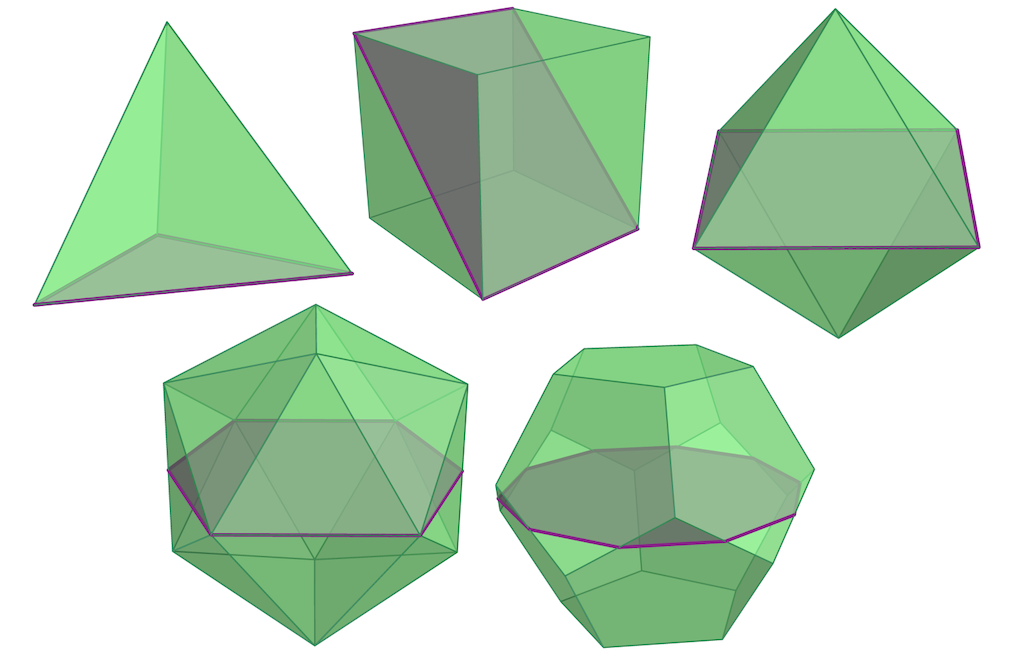
\includegraphics[width=13cm]{math_pics/polytopes.png}
	\caption{Polytopes \cite{Brandenburg2024}}
\end{figure}
Now, if their vertices are exactly at the integer Cartesian coordinates, then they are called \textbf{integer polytopes}, meaning the polytope itself is the \textbf{convex hull} of the integer points inside it.

Now we can use this to asymptotically analyze multivariate polynomials, by looking at the \textbf{Newton polytope} of the polynomial, which is the convex hull of the integer points in $\mathbb{R}^n$ corresponding to the monomials of the polynomial.

Taking a vector $y = (y_1, \ldots, y_n)$, and $(a_k)_k \subseteq \mathbb{N}^n$ pair-wise distinct, consider
\[
 f(y) = \sum_{k} c_k y^{a_k}
\]
where $(x_1, \ldots, x_n)^{(y_1, \ldots, y_n)}$ is a representation of the monomial $x_1^{y_1} x_2^{y_2} \ldots x_n^{y_n}$.
Now, the \textbf{Newton polytope} of that polynomial is.
\[
	\mathrm{Newt}(f)=\left\{\sum_k\alpha_k\mathbf{a}_k \middle|\sum_k\alpha_k=1\And\forall j\alpha_j\geq0\right\}, \forall c_k \neq 0_n
\]
This structure offers a lot in insight into where (or if) roots might be.
Take now, the Newton Polytope of $\det G_6(h)$, which by using software like \href{https://polymake.org/doku.php/start}{Polymake}\footcite{Assarf2017, Gawrilow2000} we can obtain its hyper-plane intersection form
% create matrix with no borders like no parantheses, just like a table
\begin{align*}
	\left.
	\begin{array}{ccc}
		-h_{1} \geq -6 &
		-h_{1} - h_{2} \geq -11 &
		-h_{1} - h_{2} - h_{3} \geq -15 \\
		-h_{1} - h_{2} - h_{3} - h_{6} \geq -18 &
		h_{6} \geq 0 &
		-h_{2} \geq -6 \\
		-h_{1} - h_{3} \geq -11 &
		-h_{3} - h_{6} \geq -11 &
		-h_{2} - h_{3} - h_{6} \geq -15 \\
		-h_{1} - h_{3} - h_{6} \geq -15 &
		h_{1} \geq 0 &
		-h_{2} - h_{3} \geq -11 \\
		-h_{2} - h_{6} \geq -11 &
		-h_{1} - h_{2} - h_{6} \geq -15 &
		-h_{3} \geq -6 \\
		h_{2} \geq 0 &
		-h_{1} - h_{6} \geq -11 &
		-h_{6} \geq -6 \\
		h_{3} \geq 0
	\end{array} \right.
\end{align*}
By treating $G_6(h)$ like an $h_1, h_2, h_3 \text{ and }, h_6$ polynomial, we observe the factor
\[
	h_{10}h_7 - h_8 h_9
\]
pops out. Now we might want to make the monomials whose factors are that, dominant, by performing the restriction / transformation;
\begin{equation}\label{h_substitution}
	h_1\to t,h_2\to t,h_3\to t,h_6\to t.
\end{equation}
Now we represent $\det G_6(h)$ as a polynomial of variable $t$ with coefficients in all other h's:
\begin{equation}\label{6th_hurwitz_det}
	\begin{aligned}
		\det G_6(t)
		&=324t^{18}(h_{10}+h_7)(h_{10}h_7-h_8h_9)+\ldots\\&+h_{10}h_4h_5h_7h_8h_9\\&\cdot(h_{10}+h_4)(h_{10}+h_5)(h_{10}+h_7)(h_{10}+h_8)(h_{10}+h_9)\\&\cdot(h_4+h_5)(h_4+h_7)(h_4+h_8)(h_4+h_9)\\&\cdot(h_5+h_7)(h_5+h_8)(h_5+h_9)\\&\cdot(h_7+h_8)(h_7+h_9)\\&\cdot(h_8+h_9).
	\end{aligned}	
\end{equation}
Since the only $minuses$ that might pollute its positivity are in the "$324 t^{18}$" term $\implies \det G_6(0) > 0$, so if
\begin{gather}\label{bif_ineq_condition}
	h_{10}h_{7} - h_{8}h_{9} < 0 \\
	\Downarrow \notag \\
	\exists t_1 > 0 : \det G_6(t_1) = 0, \det G_6(t) < 0, \forall t > t_1 \notag
\end{gather}
by the Intermediate Value Theorem, meaning it passes $0$.

So it means we've shown a root exists for $\det G_6(h)$, and hence a Hopf bifurcation may occur in the system.

Where though? This is where the second part of the problem comes in.

\begin{itemize}
	\item \rom{1} We may experimentally just pick and choose values that verify	\ref{bifurcation_main_condition} and \ref{bif_ineq_condition}, for exmaple, \cite{conradi2024} did $ h_9 = 2, h_8 = h_7 = h_{ 10 } = 1$
	\item \rom{2} $\forall h_4, h_5 > 0$, like $h_5 = h_4 = 1$
	\item \rom{3} Now taking \ref{h_substitution} along with the previous values and using them in \ref{6th_hurwitz_det} we get
		\begin{gather*}
			497664+10946304t+103721056t^{2}+579850652t^{3}+2169242876t^{4} \\
			+5787611019t^{5}+113986711182t^{6}+16865933820t^{7} \\
			+18863357157t^{8}+15900121640t^{9}+9989687485t^{10} \\
			+4589099030t^{11}+1497364081t^{12}+331280824t^{13} \\
			+45135703t^{14}+2794428t^{15}-85122t^{16}-20304t^{17}-648t^{18}=0	
		\end{gather*}
	\item \rom{4} Now taking its root $\implies t^* \approx 14.8$
	\item \rom{5} Using these to verify \ref{bifurcation_transversality_condition}:
		\begin{align*}
			h^* =
			\begin{pmatrix}
				14.8 \\
				14.8 \\
				14.8 \\
				1 \\
				1 \\
				14.8 \\
				1 \\
				1 \\
				2 \\
				1
			\end{pmatrix}
		\end{align*}
	\item \rom{6} Taking $t > t^*$, say $15$, and solving for \ref{k_convert_back_from_convex} and $x = \frac{1}{h}$:
		\begin{align}
			h &= \left(15,15,15, 1,1,15,1,1,2,1\right)^T \\
			x &= \left( \frac{1}{15},\frac{1}{15},\frac{1}{15},1,1,\frac{1}{15},1,1,\frac{1}{2},1 \right)^T \\
			k &= \left( 225 \lambda, \lambda, 15\lambda, 225\lambda, \lambda, 15\lambda, 2\lambda  \right) \\
			&= (t^{2},1,t,1,t^{2},1,t,2)
		\end{align}
\end{itemize}
Considering $\lambda = 1$ and putting these into \href{https://github.com/viktorashi/Open-CoNtRol}{the app} we get something that looks like:
\begin{figure}[H]
	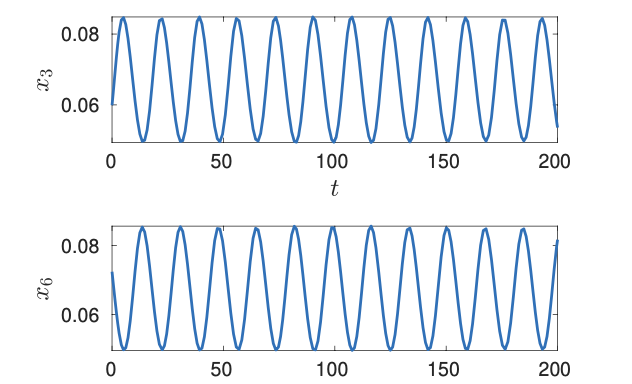
\includegraphics[width=13cm]{math_pics/oscillations.png}
	\centering
	\label{fig:x3_x6_osccilations}
	\caption{Oscillations of $S00, S11$}
\end{figure}

They're oscillating! We've found a bifurcation point!

But wait, in the beginning we reduced our system from \ref{network2} to \ref{network2_irr}, taking the reversible reactions with us. But luck would have it that \cite{banaji2017} shows that adding a reaction who's reaction vector is a linear combination of the other reactions, and hence preserves rank$\Gamma$ does, in fact mean the resulting system preserves its capacity for bifurcations.

So adding back
\begin{gather*}
	KS_{00} \xrightarrow{k_2} K \\
	KS_{10} \xrightarrow{k_5} S_{10} + K \\
	FS_{11} \xrightarrow{k_8} S_{11} + F \\
	FS_{01} \xrightarrow{k_{11}} S_{01} + F
\end{gather*}
Into our system, we obtain bifurcation parameters and initial conditions for which oscillations occur, namely:
\[
	x =
	\begin{bmatrix*}
		0.0885267\\
		0.0528367\\
		0.0496013\\
		0.74587\\
		1.261\\
		0.084892\\
		0.97124\\
		1.0069\\
		0.49383\\
		1.02
	\end{bmatrix*}
\]
and $k$ as before, but with the extra reaction rates being simply a constant we can vary to see how the system looks $k_b = k_5 = k_2 = k_{11} = k_8$. Thus we get:

\begin{figure}[H]
	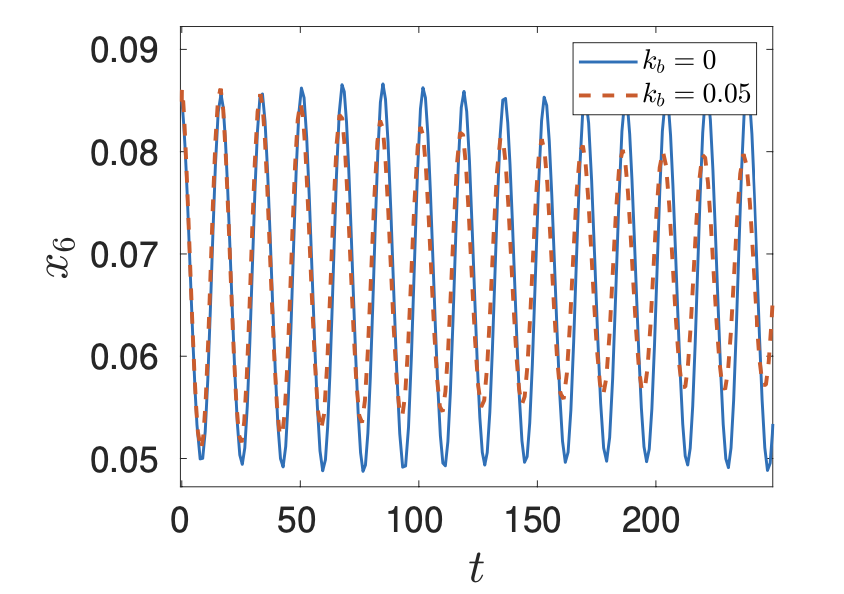
\includegraphics[width=13cm]{math_pics/oscillations-full-network.png}
	\centering
	\label{fig:full_net_oscillations}
	\caption{Oscillations of the full \ref{network2} network}
\end{figure}

There we have, a "visual" proof, you could say.

\hfill\break
\hfill\break

\textbf{Example 3}:
Now let us apply the same intuition for the following cyclic network (\ref{network3}).

\begin{figure}[H]
	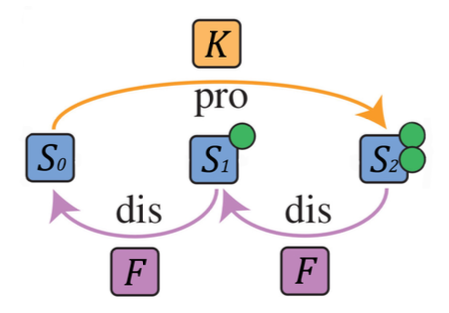
\includegraphics[width=13cm]{math_pics/ex3-bifurcations.png}
	\centering
\end{figure}

Its chemical reaction network is:
\begin{align}\label{network3}
	S_{0} + K \xrightleftharpoons[ k_2 ]{k_1} KS_{0} \xrightarrow{k_3} K S_1 \xrightleftharpoons{k_4} S_2 + K \tag{$\mathcal{N}_3$} \\
	S_{2} + F \xrightleftharpoons[ k_6 ]{k_5} FS_{2} \xrightarrow{k_7} S_1 + F \xrightleftharpoons[k_9]{k_8} FS_1 \xrightarrow{k_{10}} S_0 + F \notag
\end{align}

By the same results used in \ref{network2}, we go $1$ level up the simplification stack, removing the reversible reactions and re-naming the reaction constants $k_i$ like so:
\begin{align}\label{network3_irr}
	S_{0} + K \xrightarrow{k_1} KS_{0} \xrightarrow{k_2} K S_1 \xrightarrow{k_3} S_2 + K \tag{$\mathcal{N}_3 / IR $} \\
	S_{2} + F \xrightarrow{k_4} FS_{2} \xrightarrow{k_5} S_1 + F \xrightarrow{k_6} FS_1 \xrightarrow{k_{7}} S_0 + F \notag
\end{align}

By the results used previously, we find that if this network is to have bifurcations, then adding the inverse reactions back would mean \ref{network3} also does. Going up $1$ more level, using \textbf{Theorem 3.2} from \cite{banaji2017} we see that performing a stoichiometry matrix rank preserving operation of removing species $S_1$ and $K$, then we get network:
\begin{align}\label{network3_irr_s}
	S_{0} \xrightarrow{k_1} KS_{0} \xrightarrow{k_2} K S_1 \xrightarrow{k_3} S_2 \tag{$\mathcal{N}_3 / IR / S$} \\
	S_{2} + F \xrightarrow{k_4} FS_{2} \xrightarrow{k_5} F \xrightarrow{k_6} FS_1 \xrightarrow{k_{7}} S_0 + F \notag
\end{align}

which - as previously - if it's to admit bifurcations, then \ref{network3_irr} would have them as well.

And finally, removing the $2$ complexes $FS_1$,$KS_0$ and their corresponding $2$ reactions through a simmilar opperation \cite{banaji2017}, this time dipping from rank $\Gamma_{\text{\ref{network3_irr_s}}}$ = 6 to rank $\Gamma_{\text{\ref{network3_irr_ss}}}$ = 4
\begin{align}\label{network3_irr_ss}
	S_{0} \xrightarrow{k_1} KS_{1} \xrightarrow{k_2} S_2 \tag{$\mathcal{N}_3 / IR / SS$} \\
	S_{2} + F \xrightarrow{k_3} FS_{2} \xrightarrow{k_4} F \xrightarrow{k_{5}} S_0 + F \notag
\end{align}

We get the system which we'll end up analysing, again, as before knowing that if we are to find a bifurcation in \ref{network3_irr_ss} - this extra-extra simplification - then that would also be the case for \ref{network3_irr_s} $\implies$ \ref{network3_irr} $\implies$ \ref{network3}.

(\ref{network3_irr_ss})'s system of equations is:
\begin{equation}\label{last_dyn_sys}
	\begin{aligned}&\dot{x}_1(t)=-k_1x_1(t)+k_5x_4(t)\\&\dot{x}_2(t)=k_1x_1(t)-k_2x_2(t)\\&\dot{x}_3(t)=k_2x_2(t)-k_3x_3(t)x_4(t)\\&\dot{x}_4(t)=-k_3x_3(t)x_4(t)+k_4x_5(t)\\&\dot{x}_5(t)=k_3x_3(t)x_4(t)-k_4x_5(t).
	\end{aligned}
\end{equation}
Using \ref{jacobian_convex_params} to get the convex-parametered Jacobian:
\[
	J_{\text{\ref{network3_irr_ss}}}(h,\lambda)=
	\begin{bmatrix}-\lambda h_{1}&0&0&\lambda h_{4}&0\\\lambda h_{1}&-\lambda h_{2}&0&0&0\\0&\lambda h_{2}&-\lambda h_{3}&-\lambda h_{4}&0\\0&0&-\lambda h_{3}&-\lambda h_{4}&\lambda h_{5}\\0&0&\lambda h_{3}&\lambda h_{4}&-\lambda h_{5}
	\end{bmatrix}.
\]
And its char. poly.:
\[
	det(zI-J_A(h,\lambda))=z[a_0(h,\lambda)z^4+a_1(h,\lambda)z^3+a_2(h,\lambda)z^2+a_3(h,\lambda)z+a_4(h,\lambda)].
\]
We may find that this is also a network with only one extreme ray, namely $E^T = \left(1,1,1,1,1\right)$. Using
\[
	v(k,x^*)=(k_1x_1,k_2x_2,k_3x_3x_4,k_4x_5,k_5x_4)^T.
\]
into \ref{flux_cone} $\implies$
\[
	k_1x_1=k_2x_2=k_3x_3x_4=k_4x_5=k_5x_4=\lambda.
\]
We can flip these around like so
\begin{equation}\label{last_jacobian}
	x_{1}=\frac{\lambda}{k_{1}},x_{2}=\frac{\lambda}{k_{2}},x_{3}=\frac{\lambda}{k_{3}x_{4}},x_{4}=\frac{\lambda}{k_{5}},x_{5}=\frac{\lambda}{k_{4}}.
\end{equation}

And only couting $x_4 = \frac{\lambda}{k_5}$ as a principal, we get $\lambda = k_5 x_4 \implies$
\begin{equation}\label{last_char_poly}
	x =
	\left(\frac{k_5x_4}{k_1},\frac{k_5x_4}{k_2},\frac{k_5}{k_3},x_4,\frac{k_5x_4}{k_4}\right).	
\end{equation}
We can get our $k$'s from \ref{k_convert_back_from_convex}
\begin{gather*}
	k =
	\left(h_1 \lambda, h_2 \lambda, h_3 h_4 \lambda, h_5 \lambda, h_4 \lambda\right), \\
	\left(h_1, h_2, h_3, h_4, h_5\right)
	= h = \frac{1}{x}
\end{gather*}
Take \ref{last_dyn_sys}, \ref{last_jacobian}, \ref{last_char_poly} and considering $\lambda^*$, $h^* :$
\begin{itemize}
	\item \rom{1} $\det H3(h^*, \lambda^*) = 0 \text{ and } a4(h^*, \lambda^*) > 0,$
	\item \rom{2} $\det H_1(h^*,\lambda^*)>0\quad\mathrm{and}\quad\det H_2(h^*,\lambda^*)>0,$

		With $H_i$ being the Hurwitz matrices coming from $a_0(h,\lambda^*), \ldots, a_4(h, \lambda^*)$ of \ref{last_char_poly}.
		Then $\exists$ simple Hopf bifurcaton $\forall \lambda>0$ at $h = h^*$ if, as well:

	\item \rom{3} $\exists i\in\{1,\ldots,5\}\text{ s.t. }\left.\frac{\partial\det H_3(h,\lambda)}{\partial h_i}\right|_{(h^*,\lambda)}\neq0.$ (transversality)
\end{itemize}

Well, for one, we know that
\[
	\forall h > 0 : a_{0}(h,\lambda)>0,\ldots,a_{4}(h,\lambda)>0\quad \text{ and } \quad\det H_{1}(h,\lambda)>0,\det H_{2}(h,\lambda)>0.
\]
All that's left is $H_3$. Treating $\lambda, h_3, h_4 > 0$ as some constants and $h_2 = h_5 = h_1 = t \implies h(t)^T = (t,t,h_3,h_4,t)$ we get
\begin{align*}
	\det \text{H}_3 &=
	t^2 \lambda^6
	(
		8t^4 + 24t^3h_3 + 16t^3h_4 + 24t^2h_3^2 + \\
		23t^2h_3h_4+ 10t^2h_4^2 + 8th_3 \\
		+ 10th_3^2h_4 + 4th_3h_4^2 +
		2th_4^3 - h_3h_4 - 2h_3^2h_4^2 - h_3h_4^3
	) \\
	&= 	t^2 \lambda^6 \cdot g(t)
\end{align*}
By the same logic as in \ref{bif_ineq_condition}, noticing $\frac{ d g(t) }{dt} > 0, \forall t > 0,  g(0) < 0, \lim_{t \rightarrow \infty}  g(t) = \infty \implies \exists t_1 > 0 \text{ s.t. }  g(t_1) = 0$.
Also, $\frac{d  \det \text{H}_3(t) }{dt} = 2 t \lambda^6 g(t) + t^2 \lambda^6 g'(t) \implies \frac{d  \det \text{H}_3(t) }{dt} |_{t = t_1}  = t_1^2 \lambda^6 g'(t_1) > 0,$ since $t_1 > 0; \lambda > 0$ and $g'(t_1) > 0$

Meaning \ref{network3_irr_ss} undergoes a simple Hopf bifurcation for that $t_1$ and $\forall \lambda > 0$ and some $h_3, h_4 > 0$ fixed.

In the section \ref{last_system_init_cond}, I'm plotting this sytem using \href{https://github.com/viktorashi/bachelor-thesis.git}{the app} for some initial conditions and rate constants, found simmilarly to \ref{network2}, as you can see, these also admit oscillations.

Now we know system \ref{network3_irr_ss} undergoes bifurcations, which means \ref{network3_irr_s}, \ref{network3_irr} and \ref{network3} all do, respectively.
